\documentclass[aspectratio=32]{beamer}

\usepackage{beamerthemesplit}
\usetheme{Boadilla}
\usecolortheme{dolphin}
\usefonttheme{serif}

\usepackage{multirow}
\usepackage{subfig}
\usepackage{amssymb,amsmath,mathtools}
\usepackage{amsfonts,booktabs}
\usepackage{lmodern,textcomp}
\usepackage{color}
\usepackage{tikz}
\usetikzlibrary{arrows.meta,calc,positioning,shapes.geometric}
\usepackage{multicol}
\usepackage{graphicx}
\usepackage{ctex}
\usepackage{hyperref}
\usepackage{nicefrac}
\usepackage{tabularx}
\usepackage{ragged2e}

\graphicspath{{material/}}

\setbeamertemplate{navigation symbols}{}
\setbeamertemplate{caption}[numbered]
\setbeamercolor{structure}{fg=blue!70!black}
\setbeamercolor{frametitle}{fg=blue!70!black}
\setbeamerfont{frametitle}{size=\large}
\setlength{\parskip}{2pt}
\setlength{\tabcolsep}{5pt}

\definecolor{LectureBlue}{RGB}{18,18,150}
\definecolor{SoftBlue}{RGB}{235,240,255}
\definecolor{SoftRed}{RGB}{255,239,239}
\definecolor{SoftGreen}{RGB}{235,249,240}
\setbeamercolor{lecturesection}{fg=white,bg=LectureBlue}

\newcommand{\E}{\mathbb{E}}
\newcommand{\dd}{\mathrm{d}}
\newcommand{\TFP}{\mathrm{TFP}}
\newcommand{\lecturesectionpage}[1]{%
\begin{frame}[plain]
\begin{center}
\vfill
\begin{beamercolorbox}[wd=0.74\textwidth,rounded=true,shadow=true,center,sep=1em]{lecturesection}
\LARGE #1
\end{beamercolorbox}
\vfill
\end{center}
\end{frame}
}

\title[Lecture 2: 生产函数]{Lecture 2：生产函数}
\author{陈宠\inst{1}}
\institute{中国人民大学经济学院\inst{1}}
\date{2026年秋季}

\begin{document}

\begin{frame}
\maketitle
\end{frame}

\begin{frame}{目录}
\tableofcontents[hideallsubsections]
\end{frame}

\section{增长、创新与全要素生产率}
\begin{frame}
\begin{center}
    \begin{minipage}{1\textwidth}
	\setbeamercolor{mybox}{fg=white, bg=black!50!blue}
		\begin{beamercolorbox}[wd=0.7\textwidth, rounded=true, shadow=true]{mybox}
			\LARGE \centering 增长、创新与全要素生产率
		\end{beamercolorbox}
    \end{minipage}
\end{center} 
\end{frame}

\begin{frame}{经济增长、技术创新与全要素生产率（TFP）提高：辨析}
\begin{center}
\begin{block}{课堂小问}
从直觉上来说，经济增长、技术创新与全要素生产率（生产效率）提高有什么异同？
\end{block}
\end{center}
\end{frame}



\begin{frame}{经济增长、技术创新与全要素生产率（TFP）提高：辨析}
\small
\begin{tabularx}{\textwidth}{>{\raggedright\arraybackslash}p{2.5cm}
    >{\raggedright\arraybackslash}X >{\raggedright\arraybackslash}X}
\toprule
概念 & 经济含义 & 常见测度 \\
\midrule
经济增长
& 经济总量增加：产出、GDP、增加值，甚至灯光亮度
& $\Delta Y/Y$、人均 GDP 增长率、每工时产出增长率 \\
\addlinespace
技术创新
& 发明、改进并采用新的产品、工艺或组织方式
& 专利数量、专利质量、研发支出、新产品或新工艺采用 \\
\addlinespace
全要素生产率提高
& 给定可观测投入下，生产系统把投入转化为产出的效率
& 由生产函数和数据反推出的残差\\
\bottomrule
\end{tabularx}
\vspace{0.35cm}
\begin{alertblock}{警告：创新与TFP并不等价}
在许多经济学论文中，我们总是混用创新和全要素生产率的概念，但实际上这并不是正确的。在实践中,全要素生产率经常可以测度出降低，但是技术退步通常是难以理解的。
\end{alertblock}
\end{frame}

\section{生产函数：从故事到抽象}
\begin{frame}
\begin{center}
    \begin{minipage}{1\textwidth}
	\setbeamercolor{mybox}{fg=white, bg=black!50!blue}
		\begin{beamercolorbox}[wd=0.7\textwidth, rounded=true, shadow=true]{mybox}
			\LARGE \centering 生产函数：从故事到抽象
		\end{beamercolorbox}
    \end{minipage}
\end{center} 
\end{frame}


\begin{frame}{采集经济}
\begin{block}{故事设定}
\begin{itemize}
    \item 考虑一个原始部落，每年部落需要靠采摘果实为生
    \item 果实的存量对于部落中的人口来说是非常多的
    \item 部落中每派一个劳动力\(L_t\)出门采摘果实，便获得一颗果实
\end{itemize}
\end{block}
\[
Y_t=L_t
\]
\begin{block}{加入效率(全要素生产率)}
    如果部落中劳动率的采摘效率提高了：每个劳动力能够采摘两颗果实
\end{block}
\[
Y_t=A_{t} \times L_{t},A_{t}=2
\]
\end{frame}

\begin{frame}{种植经济:引入资本}
\begin{block}{故事设定}
\begin{itemize}
    \item 考虑一个原始村落，每年部落需要种田为生
    \item 土地对于村落中的人口来说是非常多的
    \item 部落中每投入一单位种子\(K_t\)，并派一个劳动力\(L_t\)，便获得一单位产出\footnote{为了简化起见，我们假定产出就是“种子”}
\end{itemize}
\end{block}
\[
Y_t=K_t \times L_t
\]

\begin{block}{加入效率(全要素生产率)}
    如果村落中种植效率提高了：一组投入可以获得两颗种子
\end{block}
\[
Y_t=K_t \times L_t \times A_{t},A_{t}=2
\]
\end{frame}

\begin{frame}{种植经济：生产动态}
\begin{block}{吃种子、存种子\(\Longrightarrow\)一般均衡}
\[
C_t+I_t=Y_t
\]
\end{block}

\begin{block}{种子数量的迭代\(\Longrightarrow\)资本积累方程}
\begin{center}
\begin{tikzpicture}[>=Stealth, every node/.style={font=\small}]
\draw[->, thick] (0,0) -- (10.2,0);
\foreach \x/\lab in {0/$t$,3.2/$t+1$,6.4/$t+2$,9.6/$t+3$}
    \draw (\x,0.12)--(\x,-0.12) node[below=0.15cm] {\lab};
\node[draw=LectureBlue, fill=SoftBlue, rounded corners, align=center]
    at (1.6,1.05) {$K_t$\\资本存量};
\node[draw=LectureBlue, fill=SoftGreen, rounded corners, align=center]
    at (4.8,1.05) {$I_t$\\当期投资};
\node[draw=LectureBlue, fill=SoftBlue, rounded corners, align=center]
    at (8.0,1.05) {$K_{t+1}$\\下一期资本};
\draw[->, thick] (2.9,1.05) -- (3.6,1.05);
\draw[->, thick] (6.1,1.05) -- (6.8,1.05);
\end{tikzpicture}
\end{center}
\vspace{0.25cm}
\[
K_{t+1}=I_t+(1-\delta)K_t
\]
\end{block}

\begin{itemize}
    \item 每期的产出会发生什么样的变化？
\end{itemize}
\end{frame}


\begin{frame}{走进更一般的生产函数形式}
\begin{columns}[T]
\begin{column}{0.49\textwidth}
\[
Y_t=F(A_t,K_t,L_t,\ldots)
\]
\vspace{0.15cm}
\begin{tikzpicture}[>=Stealth, scale=0.75, transform shape, node distance=0.75cm,
    every node/.style={font=\small},
    input/.style={draw=LectureBlue, fill=SoftBlue, rounded corners,
        minimum width=1.6cm, minimum height=0.55cm, align=center},
    output/.style={draw=LectureBlue, fill=SoftGreen, rounded corners,
        minimum width=2cm, minimum height=0.65cm, align=center}]
\node[input] (k) {$K$};
\node[input, below=of k] (l) {$L$};
\node[input, below=of l] (a) {$A$};
\node[output, right=1.15cm of l] (f) {$F(\cdot)$};
\node[output, right=1.15cm of f] (y) {$Y$};
\draw[->] (k) -- (f);
\draw[->] (l) -- (f);
\draw[->] (a) -- (f);
\draw[->, thick] (f) -- (y);
\end{tikzpicture}
\end{column}
\begin{column}{0.46\textwidth}
\footnotesize
\begin{itemize}
    \item $K$：物质资本；
    \item $L$：劳动投入及其质量；
    \item $A$：效率、技术或其他未观测因素；
    \item $\ldots$：土地、中间品、组织、制度和人力资本等。
\end{itemize}
\vspace{0.2cm}
\end{column}
\end{columns}
\end{frame}

\section{生产函数估计与TFP测度}
\begin{frame}
\begin{center}
    \begin{minipage}{1\textwidth}
	\setbeamercolor{mybox}{fg=white, bg=black!50!blue}
		\begin{beamercolorbox}[wd=0.7\textwidth, rounded=true, shadow=true]{mybox}
			\LARGE \centering 生产函数估计与TFP测度
		\end{beamercolorbox}
    \end{minipage}
\end{center} 
\end{frame}

\begin{frame}{生产函数估计：一个简介}
\begin{block}{课堂小问}
如果我们有足够多的所有可观测数据：\(Y_t,K_t,L_t,\ldots\)。我们怎么才能得到生产函数的形式
\end{block}
\end{frame}

\begin{frame}{流派一：非参数估计}
\begin{block}{核心思想}
\begin{itemize}
    \item 不预先设定函数形式，让数据说话
    \item 适当加入一些约束：半参估计
\end{itemize}
\end{block}

\begin{block}{例：Nadaraya-Watson核回归}
\begin{itemize}
    \item 核心思想：在局部上使用周边观测点拟合
    \item 假设我们可以观测到产出的数值\(Y_i\)，以及投入的数值\(X_i=(K_i,L_i,\ldots)\)，那么可用局部线性核回归：
\end{itemize}
\end{block}
\[
y\left(x\right)=\arg\min_{a}\sum_{i=1}^{n}K\left(\frac{x-X_i}{h}\right)\left(Y_i-a\right)^2
\]

\[
\Longrightarrow y\left(x\right)=\frac{\sum_{i}K\left(\frac{x-X_i}{h}\right)Y_i}{\sum_{i}K\left(\frac{x-X_i}{h}\right)}
\]
\end{frame}

\begin{frame}{流派二：参数估计}
\begin{block}{参数估计中一个自然的问题}
既然可以设定函数形式，那么什么样的函数形式是好的呢？
\end{block}
\end{frame}

\begin{frame}{Kaldor典型化事实：一个选择Cobb-Douglas生产函数的理由}
\begin{block}{Kaldor典型化事实}
Kaldor(1957)发现在一个成熟的工业化国家中，大概有这些特征：
\begin{itemize}
    \item 总产出和生产率增速大体不变
    \item 人均资本量增速持续增长
    \item 实际利率大体稳定不变
    \item 资本-产出率长期不变
    \item 生产要素收入在国民收入中所占份额大体不变(*)
    \item 不同国家产出增速和劳动生产率存在显著差异
\end{itemize}
\end{block}

\begin{block}{课堂小问}
什么样的函数形式可以满足“生产要素收入在国民收入中所占份额大体不变”？
\end{block}
\end{frame}

\begin{frame}{C-D函数中的生产率估计}
\[
Y_t=A_tK_t^\alpha L_t^{1-\alpha},
\qquad 0<\alpha<1
\]

\[
\Longrightarrow \ln Y_t=\ln A_t+\alpha\ln K_t+(1-\alpha)\ln L_t
\]

\begin{itemize}
    \item 通过假设产出存在不可观测误差\(u_t\)
    \item 可以使用带约束的OLS估计\(\alpha\)
    \item 从而假设\(\ln(A_t)=a+bt\)可以被估计
\end{itemize}
\end{frame}

\section{从C-D到更一般的生产函数形式}
\begin{frame}
\begin{center}
    \begin{minipage}{1\textwidth}
	\setbeamercolor{mybox}{fg=white, bg=black!50!blue}
		\begin{beamercolorbox}[wd=0.7\textwidth, rounded=true, shadow=true]{mybox}
			\LARGE \centering 从C-D到更一般的生产函数形式
		\end{beamercolorbox}
    \end{minipage}
\end{center} 
\end{frame}

\begin{frame}{C-D函数的性质}
\begin{block}{C-D函数的数学性质}
\begin{itemize}
    \item CRS：$F(\lambda K,\lambda L)=\lambda F(K,L)$
    \item 要素份额恒定：资本份额为 $\alpha$，劳动份额为 $1-\alpha$
    \item 边际报酬递减：$MP_K=\alpha A K^{\alpha-1}L^{1-\alpha}$，$MP_L=(1-\alpha)A K^\alpha L^{-\alpha}$
    \item 替代弹性恒定为1（*）：\(\frac{\partial K/L}{\partial w/r}=1\)
\end{itemize}
\end{block}
\end{frame}

\begin{frame}{CES：替代弹性为常数的函数}
\begin{block}{课堂小问}
\begin{itemize}
    \item 要素报酬恒定是否是一个合适的假设？
    \item 替代弹性为常数是否是一个合适的假设？
\end{itemize}
\end{block}
\end{frame}

\begin{frame}{CES函数及其性质}
\[
Y_t=A_t\left[\alpha K_t^{\frac{\sigma-1}{\sigma}}+\left(1-\alpha\right)L_t^{\frac{\sigma-1}{\sigma}}\right]^{\frac{\sigma}{\sigma-1}}
\]

\begin{block}{CES函数的数学性质}
\begin{itemize}
    \item CRS：$F(\lambda K,\lambda L)=\lambda F(K,L)$
    \item 要素份额受到相对价格影响
    \item 边际报酬递减
    \item 替代弹性恒为$\sigma$
\end{itemize}
\end{block}

\begin{block}{$\sigma$的含义}
$\sigma$ 衡量资本劳动比率对边际替代率变化的反应：
$\sigma$ 越大，生产者越容易用一种要素替代另一种要素。
\end{block}
\end{frame}

\begin{frame}{Arrow et al.（1961）：从极端走向 CES}
\begin{columns}[T]
\begin{column}{0.42\textwidth}
\begin{figure}
\centering
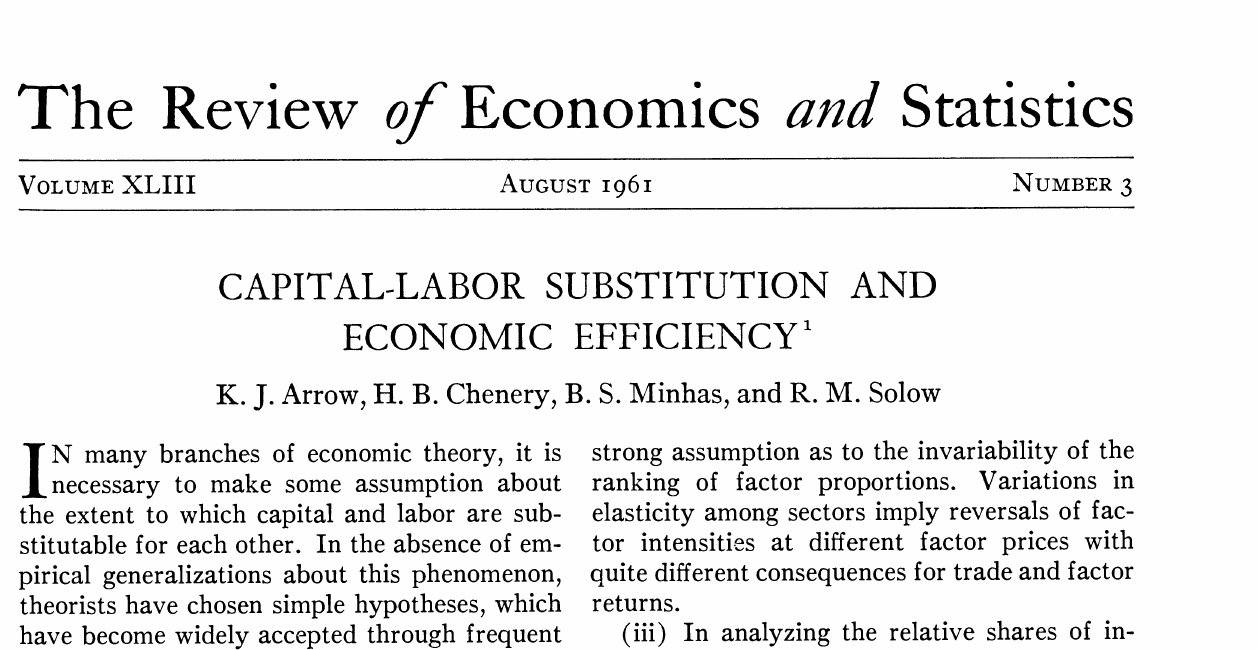
\includegraphics[width=\linewidth]{arrow1961_ces_title.png}
\caption{\scriptsize Arrow, Chenery, Minhas \& Solow (1961)}
\end{figure}
\end{column}
\begin{column}{0.53\textwidth}
\begin{itemize}
    \item Leontief：投入比例近似固定，替代弹性为 0；
    \item Cobb--Douglas：替代弹性等于 1；
    \item 完全替代：资本和劳动可以线性互换，替代弹性趋近正无穷；
\end{itemize}
\end{column}
\end{columns}

\begin{alertblock}{Arrow et al.（1961）}
CES是以上三种形式的一般形式
\end{alertblock}
\end{frame}

\begin{frame}{从 CES 恢复 Cobb--Douglas}
\small
\setlength{\abovedisplayskip}{3pt}
\setlength{\belowdisplayskip}{3pt}
令
\[
\rho\equiv\frac{\sigma-1}{\sigma},\qquad
\sigma\to1\Longleftrightarrow\rho\to0.
\]
对前文 CES 函数取对数，并将幂函数写成指数形式：
\[
\ln\frac{Y}{A}
=\frac{\ln\!\left[\alpha K^\rho+(1-\alpha)L^\rho\right]}{\rho}
=\frac{\ln\!\left[\alpha e^{\rho\ln K}
 +(1-\alpha)e^{\rho\ln L}\right]}{\rho}.
\]
当 $\rho\to0$ 时，分子和分母都趋于 $0$。因此由洛必达法则，
\[
\begin{aligned}
\lim_{\rho\to0}\ln\frac{Y}{A}
&=\lim_{\rho\to0}
\frac{\alpha K^\rho\ln K+(1-\alpha)L^\rho\ln L}
     {\alpha K^\rho+(1-\alpha)L^\rho}\\
&=\alpha\ln K+(1-\alpha)\ln L.
\end{aligned}
\]
\begin{alertblock}{结论}
\[
\lim_{\sigma\to1}Y
=A\exp{\left[\alpha\ln K+(1-\alpha)\ln L\right]}
=AK^\alpha L^{1-\alpha}.
\]
\end{alertblock}
\end{frame}

\begin{frame}{从 CES 恢复 Leontief}
\footnotesize
\setlength{\abovedisplayskip}{1.5pt}
\setlength{\belowdisplayskip}{1.5pt}
仍令 $\rho=(\sigma-1)/\sigma$。当 $\sigma\to0^+$ 时，
\[
\rho\to-\infty,\qquad
Y=A\left[\alpha K^\rho+(1-\alpha)L^\rho\right]^{1/\rho}.
\]
假定 $K,L>0$，分情形考察最小投入：
\vspace{-0.08cm}
\begin{columns}[T]
\begin{column}{0.48\textwidth}
\begin{block}{$K<L$}
\scriptsize
提取 $K^\rho$，得到
\[
\frac{Y}{A}=K\left[\alpha+(1-\alpha)
\left(\frac{L}{K}\right)^\rho\right]^{1/\rho}.
\]
因 $L/K>1$ 且 $\rho\to-\infty$，有
$(L/K)^\rho\to0$；同时 $1/\rho\to0$，所以
\[
\frac{Y}{A}\to K\alpha^0=K.
\]
\end{block}
\end{column}
\begin{column}{0.48\textwidth}
\begin{block}{$L<K$}
\scriptsize
对称地提取 $L^\rho$，得到
\[
\frac{Y}{A}
=L\left[\alpha\left(\frac{K}{L}\right)^\rho
 +(1-\alpha)\right]^{1/\rho}.
\]
此时 $(K/L)^\rho\to0$，且 $1/\rho\to0$，所以
\[
\frac{Y}{A}\to L(1-\alpha)^0=L.
\]
\end{block}
\end{column}
\end{columns}
\vspace{-0.15cm}
\begin{alertblock}{结论}
\scriptsize
若 $K=L$，则 $Y/A=K$；综合三种情形，
\[
\lim_{\sigma\to0^+}Y=A\min\{K,L\}.
\]
在这一规范化下，$\alpha$ 影响有限替代弹性下的权重，但在 Leontief 极限中消失。
\end{alertblock}
\end{frame}

\begin{frame}{从 CES 恢复完全替代}
\small
\setlength{\abovedisplayskip}{3pt}
\setlength{\belowdisplayskip}{3pt}
仍令 $\rho=(\sigma-1)/\sigma$。当 $\sigma\to\infty$ 时，
\[
\rho\to1,\qquad \frac{1}{\rho}\to1.
\]
因此 CES 函数可以直接取极限：
\[
\lim_{\sigma\to\infty}Y
=A\left[\alpha K+(1-\alpha)L\right].
\]
对极限生产函数求边际产出：
\[
MP_K=\frac{\partial Y}{\partial K}=A\alpha,
\qquad
MP_L=\frac{\partial Y}{\partial L}=A(1-\alpha).
\]
沿等产量曲线 $dY=0$，有
\[
\mathrm{MRTS}_{KL}
=\frac{MP_K}{MP_L}
=\frac{\alpha}{1-\alpha},
\qquad
L=\frac{Y/A}{1-\alpha}
 -\frac{\alpha}{1-\alpha}K.
\]
\vspace{-0.08cm}
\begin{alertblock}{结论}
等产量曲线是一条直线，MRTS 不随 $K/L$ 改变；资本和劳动可以按固定比例相互替代，因此该极限是完全替代生产函数。
\end{alertblock}
\end{frame}

\begin{frame}{用等产量曲线把三个模型放在一起}

\begin{center}
\begin{tikzpicture}[x=1.05cm,y=0.82cm]
\draw[->] (0,0) -- (5.3,0) node[right] {$K$};
\draw[->] (0,0) -- (0,4.4) node[above] {$L$};
\draw[blue!70!black, thick] plot[smooth] coordinates
    {(0.7,4.0) (1.1,2.7) (1.7,1.95) (2.5,1.35) (3.5,0.9) (4.5,0.6)};
\draw[red!70!black, thick] (0.55,3.7) -- (3.8,0.55);
\draw[green!45!black, thick] (0.8,3.6) -- (0.8,0.8) -- (4.15,0.8);
\node[blue!70!black] at (3.75,1.45) {\scriptsize $\sigma=1$};
\node[red!70!black] at (3.0,2.9) {\scriptsize $\sigma\to\infty$};
\node[green!45!black] at (1.15,1.15) {\scriptsize $\sigma\to0$};
\end{tikzpicture}
\end{center}

\begin{itemize}
    \item 曲线越弯，替代越困难；
    \item 估计 CES 的意义在于让数据决定“资本和劳动能否替代”。
\end{itemize}
\end{frame}

\begin{frame}{总结}
\begin{enumerate}
    \item 增长、创新和 TFP 必须先在概念上分开
    \item 介绍生产函数及生产函数的估计
    \item Cobb-Douglas 用 Kaldor 事实获得经验吸引力，却固定了替代弹性和收入份额
    \item CES 允许替代弹性成为参数，连接 Leontief、Cobb-Douglas 和完全替代
\end{enumerate}
\end{frame}

\begin{frame}{参考文献}
\small
\begin{thebibliography}{9}

\bibitem{arrow1961}
Arrow, K. J., Chenery, H. B., Minhas, B. S., \& Solow, R. M. (1961).
\newblock Capital-Labor Substitution and Economic Efficiency.
\newblock \emph{The Review of Economics and Statistics}, 43(3), 225--250.

\bibitem{kaldor}
Kaldor, N. (1961).
\newblock Capital Accumulation and Economic Growth.
\newblock In \emph{The Theory of Capital}.
\end{thebibliography}

\begin{center}
\makebox[\textwidth][c]{%
\begin{beamercolorbox}[
    wd=0.70\textwidth,
    rounded=true,
    shadow=true,
    center,
    sep=0.8em
]{lecturesection}
    \centering
    \Huge Thanks!\\[0.25cm]
    \large\texttt{chenchong@ruc.edu.cn}
\end{beamercolorbox}%
}
\end{center}
\end{frame}

\end{document}
